\documentclass[a4paper]{report}
\usepackage{a4wide}
\usepackage[utf8]{inputenc}
\usepackage{parskip}
\usepackage{hyperref}
\usepackage{epsfig}
\usepackage{background}
\usepackage{mathptmx}

% To avoid tikz error, see https://tex.stackexchange.com/questions/165929/semiverbatim-with-tikz-in-beamer
\makeatletter
\global\let\tikz@ensure@dollar@catcode=\relax
\makeatother

\backgroundsetup{
scale=1,
angle=0,
opacity=1,
contents={
\includegraphics[width=\paperwidth,height=\paperheight]{images/spi-front.jpg}}
}

\hypersetup{
  colorlinks   = true,
  urlcolor     = blue,
  linkcolor    = blue,
  pdfinfo = {
    Title = {SPI Annual Report 2020},
    Author = {Software in the Public Interest, Inc.},
    Keywords = {SPI, free software, open source, FOSS, annual report, charity, non-profit, 501c3},
  }
}

\begin{document}

\title{Software in the Public Interest, Inc.\\
2020 Annual Report}
\date{July XXX, 2021}

\maketitle

\newpage

\backgroundsetup{
scale=1,
angle=0,
opacity=1,
contents={
\includegraphics[width=\paperwidth,height=\paperheight]{images/spi-content.jpg}}
}

\hspace{1em}

To the membership, board and friends of Software in the Public Interest, Inc:

As mandated by Article 8 of the SPI Bylaws, I respectfully submit this annual report on the activities of Software in the Public Interest, Inc. and extend my thanks to all of those who contributed to the mission of SPI in the past year.

  \emph{-- Michael Schultheiss, SPI President}

\newpage

\tableofcontents

\newpage

\chapter{President's Welcome}
\label{sec:president}

  \emph{-- Michael Schultheiss, SPI President}

\chapter{Committee Reports}
\section{Membership Committee}

\subsection{Statistics}

On January 1, 2020 we had 222 contributing and 1138 non-contributing members.  On December 31, 2020 there were 232 contributing members and 1173 non-contributing members.  This is an increase of 10 contributing members and an increase of 35 non-contributing members.

\chapter{Board Report}
\section{Board Members}

Board members as of January 1, 2020:

\begin{itemize}
\item Michael Schultheiss (President)
\item Stephen Frost (Vice President)
\item Tim Potter (Secretary)
\item Martin Zobel-Helas (Treasurer)
\item Luca Filipozzi
\item Forrest Fleming
\item Chris Lamb
\item Héctor Orón Martínez
\item Andrew Tridgell
\end{itemize}

Board members as of December 31, 2020:

\begin{itemize}
\item Michael Schultheiss (President)
\item Stephen Frost (Vice President)
\item Tim Potter (Secretary)
\item Martin Zobel-Helas (Treasurer)
\item Joe Conway
\item Luca Filipozzi
\item Forrest Fleming
\item Chris Lamb
\item Héctor Orón Martínez
\end{itemize}

\section{Board Changes}

Changes that occurred during the year:

\begin{itemize}

\item The terms for Tim Potter and Andrew Tridgell expired in July 2020.  Tim sought, and obtained, re-election.  We'd like to thank Andrew for his work on the board.  Joe Conway joined the board as part of the same election.

\item On August 10, 2020 the board voted to appoint the following officers:

\begin{itemize}
\item President: Michael Schultheiss
\item Vice President: Stephen Frost
\item Secretary: Tim Potter
\item Treasurer: Martin Zobel-Helas
\end{itemize}

\end{itemize}

\section{Elections}

A board membership election was conducted in July 2020.  There were 2 board seats up for election.  Nominations were received from Joe Conway, Milan Kupcevic, and Tim Potter.  Joe Conway and Tim Potter were elected for a 3 year term.

\chapter{Treasurer's Report}

\section{Income Statement}

This covers the Period January 1, 2020 -- December 31, 2020

\begin{verbatim}
\end{verbatim}

\section{Balance Sheet}

\begin{verbatim}
Balance Sheet as of December 31, 2020
\end{verbatim}

\chapter{Member Project Reports}

\section{New Associated Projects}

\subsection{ns-3}

\href{https://www.nsnam.org/}{ns-3} is a discrete-event, packet-level network simulator with an emphasis on networking research and education. Users of ns-3 can construct simulations of computer networks using models of traffic generators, protocols such as TCP/IP, and devices and channels such as Wi-Fi and LTE, and analyze or visualize the results. Simulation plays a vital role in the research and education process, because of the ability for simulations to obtain reproducible results (particularly for wireless protocol design), scale to large networks, and study systems that have not yet been implemented. A particular emphasis in ns-3 is a high degree of realism in the models (including frameworks for using real application and kernel code) and integration of the tool with virtual machine environments and testbeds. Very large scale simulations are possible; simulations of hundreds of millions of nodes have been published.

\subsection{Ganeti}

\href{https://www.ganeti.org/}{Ganeti} is a virtual machine cluster management tool built on top of existing virtualisation technologies such as Xen or KVM and other open source software.

Ganeti controls:

\begin{itemize}

\item Disk creation management,
\item Operating system installation for instances (in co-operation with OS-specific install scripts), and
\item Startup, shutdown, and failover between physical systems.

\end{itemize}

Ganeti is designed to facilitate cluster management of virtual servers and to provide fast and simple recovery after physical failures using commodity hardware.

\section{Updates from Associated Projects}

\subsection{0 A.D.}

0 A.D. (pronounced ``zero ey-dee'') is a cross-platform, real-time strategy (RTS) game of ancient warfare. It is a historically-based war/economy game, in which the player must lead an ancient civilization, gather resources from the map, and raise a military force to conquer enemy factions. 0 A.D.  is open source software licensed under the GPL, and its art and sound assets are licensed under CC BY-SA. It is developed by Wildfire Games, a global community of game developers.

In 2020, a large amount of work was done to update the game's JavaScript engine to SpiderMonkey 78 and hundreds of tweaks were made for a sleeker, more balanced gameplay experience. Many GUI improvements were implemented, including building snapping, which allows buildings to be placed next to each other neatly and easily. In addition, reinforcement learning, a machine learning technique, was implemented to train the game's AI to play better.

Many art assets were added and improved as well, including reworked meshes, animations, textures and materials for a large number of units, from hoplites to siege weapons and from ships to cavalry. (Some new animations of interest were created for bears, camels and baby elephants!)

We wish to extend our thanks to our generous donors and to SPI for helping us achieve this progress.

{\em Submitted by Aviv Sharon}

\subsection{Arch Linux 32}

\href{https://archlinux32.org/}{Arch Linux 32} is a community maintained fork of the Arch Linux distribution for Intel 32-bit (IA-32) type of CPUs.

In 2020 we made many packages available on i486, preparing to get X supported in 2021 there, too.  Besides that, we followed the path of Arch Linux and changed our package compression to zstd.  Additionally, we improved our build infrastructure and monitoring infrastructure, making it more resilient against unexpected interruptions.

{\em Submitted by Andreas Baumann}

\subsection{Debian}

During 2020, the \href{https://www.debian.org/}{Debian project} faced its first year during a pandemic.  This has brought several challenges to the project and its members.

We rose up to this challenge and worked on improving our online tools, and hosted our first ever \href{https://wiki.debian.org/DebianEvents/internet/2020/MiniDebConfOnline}{online MiniDebConf} in May. Following its success, we've had further online events, including our first ever completely online \href{https://debconf20.debconf.org/}{annual DebConf} event in August.

We used the proceeds from DebConf20 to help \href{https://bits.debian.org/2020/10/debian-donation-peertube.html}{fund features in PeerTube}, which will also help us to easier host some online events in the future. We've set up our \href{https://peertube.debian.social}{own PeerTube instance}, which allows
Debian video content to have a presence on the \href{https://en.wikipedia.org/wiki/Fediverse}{fediverse}.

During 2020, we gained 26 new Debian Developers, and 46 Debian Maintainers who we hope will one day become full project members.  In terms of stable releases, we released \href{https://wiki.debian.org/DebianStretch#Release_and_updates}{two point releases for Debian 9} and \href{https://wiki.debian.org/DebianBuster#Release_and_updates}{5 point releases for Debian 10}, while we prepared the freeze towards the end of the year for our next stable release.

If you'd like to know more about what the Debian project has done over 2020, please browse the \href{https://bits.debian.org/}{Bits from Debian} site along with the Misc Developer News as sent to \href{https://lists.debian.org/debian-devel-announce/}{the debian-devel-announce list}.

{\em Submitted by Jonathan Carter}

\subsection{FFmpeg}

\href{https://www.ffmpeg.org/}{FFmpeg} is a complete, cross-platform solution to record, convert and stream audio and video. It is used as the foundation platform of many projects dealing with multimedia, both open source and proprietary, and is used extensively by several web-based multimedia conversion and processing services.

In the year 2020 FFmpeg delivered a new formal release (4.3) and many security updates of old releases. A complete list of changes can be found in \href{https://git.ffmpeg.org/gitweb/ffmpeg.git/blob/HEAD:/Changelog}{the changelog}.  Also, as usual, FFmpeg joined the GSoC program, with total of \href{https://trac.ffmpeg.org/wiki/SponsoringPrograms/GSoC/2020/Results}{six assigned projects}.

Due to the pandemic crisis, no meetings and conferences were attended by FFmpeg developers during the year.

{\em Submitted by Carl Eugen Hoyos}

\subsection{Ganeti}

\href{https://ganeti.org/}{Ganeti} has achieved several important community goals in the last year: not only did the development process gain traction, we also managed to put out the first major release as a community without direct involvement from Google. This brought us the transition to Python 3, adaptations to build- and runtime dependencies of current and upcoming Linux distribution releases and many smaller fixes and improvements. We are looking forward to (re-)attract even more Ganeti developers and users and to ship new features in regular releases. We would like to thank both Google and SPI: for being the old and new home of this project!

{\em Submitted by Rudolph Bott}

\subsection{GNU TeXmacs}

Most work on \href{https://www.texmacs.org/}{TeXmacs} during the year 2020 has been focused on preparing the next major stable release 2.1.  Many bugs were fixed and the converters for LaTeX and HTML were further improved.

{\em Submitted by Joris van der Hoeven}

\subsection{LibreOffice}

In 2020, \href{https://www.libreoffice.org/}{LibreOffice} celebrated its tenth birthday. Two new major versions of the office suite introduced a variety of new features, while minor releases helped to improve stability as well. On January 29 2020, LibreOffice 6.4 was officially released after six months of work. Developers in the ecosystem and community volunteers worked on many new features. For instance, a QR Code generator was added to the suite, making it easy to add QR codes to documents (which can be read by mobile devices).  Hyperlink context menus were unified throughout the software, while a new Automatic Redaction feature was added to hide classified or sensitive data in a document based, on text or regular expression matches.

Later in the year, on August 5 2020, LibreOffice 7.0 was released.  OpenDocument, LibreOffice's native open and standardised format for office documents, was updated to version 1.3 as an OASIS Technical Committee Specification. Important new features include digital signatures and OpenPGP-based encryption of XML documents, with improvements in areas such as change tracking, and additional details in the description of elements in first pages, text, numbers and charts.  Additionally, support for Skia graphics engine was added, along with a wide range of compatibility improvements.

{\em Submitted by Sophie Gautier}

\subsection{ns-3}

\href{https://www.nsnam.org/}{ns-3} is a discrete-event, packet-level network simulator with an emphasis on networking research and education.  Our project's most notable event in 2020 was receiving the ACM SIGCOMM Networking Systems Award in recognition of the impact that ns-3 and its predecessors have contributed to the field.  We also participated in Google Code-In and Google Summer of Code, and held our annual workshop in June as a virtual event due to the pandemic.  We made two software releases with various extensions and improvements to the simulator's wireless and TCP/IP models.

{\em Submitted by Tom Henderson}

\subsection{Open Bioinformatics Foundation}

The \href{https://www.open-bio.org/}{Open Bioinformatics Foundation} (OBF) is led by a Board that elects its members. In 2020, one Board member (Yo Yehudi) finished her term and left the Board. Hilmar Lapp stepped down after 8 years as President and was elected to an At-Large seat. Peter Cock was elected as the new President, and Heather Wiencko was elected as Treasurer, replacing previous Treasurer Peter Cock.

We expanded the OBF Travel Fellowship program (now renamed to \href{https://www.open-bio.org/event-awards/}{OBF Event Fellowships}) to cover costs associated with participating in online events, in response to the global shift in event format in the year 2020.  Applications are now reviewed with a standard rubric and without the applicants' names, to reduce the chance of unintentional reviewer bias. In 2020, 7 people were awarded funds to attend in-person or virtual events. We also developed an OBF-wide Code of Conduct that applies to in-person and virtual events organised and led by OBF, and can be adopted by member projects if they choose.

OBF's flagship event is the annual Bioinformatics Open Source Conference (BOSC). Most years, BOSC has been part of the Intelligent Systems for Molecular Biology (ISMB) conference, but in 2018, and again in 2020, BOSC partnered with the Galaxy Community Conference (GCC). The 2020 conference, called the \href{https://bcc2020.github.io/}{Bioinformatics Community Conference} (BCC2020), was fully online and global, with timezone support for APAC and North America. More than 800 people from 61 countries registered for at least part of BCC2020. BOSC 2021 will be part of ISMB/ECCB 2021 Online.

{\em Submitted by Heather Wiencko}

\subsection{Open MPI}

The \href{https://www.open-mpi.org/}{Open MPI} community is a collection of academics, researchers, and vendors who continue to develop cutting-edge technology for today's most-demanding High Performance Computing (HPC) environments.

The community was hard at work throughout 2020.  We finalized the v3.0.x and v3.1.x series with the v3.0.6 and v3.1.6 releases, respectively.  We also released v4.0.3, v4.0.4, and v4.0.5 in 2020.  The community also introduced the v4.1.x series; v4.1.0 included several new features, most of which were back-ported from our main development branch because the v5.0.0 release is taking longer than expected.  The v5.0.0 release continues to be a major focal point of development: it contains several foundational changes to Open MPI's architecture, and has required extensive cross-organizational collaboration and development.  The v5.0.x series will include major new features and will be a significant milestone in the Open MPI release history.  In a perfect world, v5.0.0 will be released in 2021.

Additionally, the Hardware Locality (\texttt{hwloc}) sub-project had three maintenance subreleases of its package in 2020 (v2.2.0, v2.3.0, and v2.4.0), mainly dealing with updates for new hardware and vendor form factors in advanced computing platforms.

{\em Submitted by Jeff Squyres}

\subsection{Performance Co-Pilot}

The \href{https://pcp.io/}{PCP project} had a busy year in 2020 in spite of the pandemic.  We created seven releases throughout the year with a focus on bug fixes and stability of the v5 release from 2019.  We participated as a Google Summer of Code mentor organization for our fifth year and took on a Google Season of Docs project for the first time.  The \texttt{grafana-pcp} subproject matured with two major releases and an official \texttt{ansible-pcp} subproject was also launched this year.

{\em Submitted by Nathan Scott}

\subsection{systemd}

In 2020 we published three major releases of \href{https://systemd.io/}{systemd}. We merged 4878 commits (up from 4198 in 2019) from a total of 370 contributors. 1949 pull requests were applied.

At devconf.cz 2020 and FOSDEM 2020 the systemd project met for BoF sessions.

{\em Submitted by Lennart Poettering}

\subsection{The Mana World}

\href{https://www.themanaworld.org/about}{The Mana World} (TMW) is an effort to create an innovative free and open source MMORPG (massively multiplayer online role-playing game), along with the accompanying game engine, game client, tooling and documentation. 2020 has been an unusually slow year for us, in part due to the global health crisis we're facing. Under these circumstances, the release of our Evol-Hercules-based game server is on hold indefinitely. In 2020, we updated the look and feel of \href{https://wiki.themanaworld.org/}{our wiki}, while also improving the documentation, and removing localization for languages that were no longer maintained. Additionally, we started the process of reorganizing the operational structure of TMW (as one organization that oversees several related subprojects) to allow for greater autonomy and more flexible management of \href{https://gitlab.com/themanaworld}{our subprojects}. In continued collaboration with \href{https://moubootaurlegends.org/en/}{Moubootaur Legends}, we moved development of our \href{https://gitlab.com/themanaworld/manaplus/manaplus}{common game client} in-house as a new subproject of The Mana World.

{\em Submitted by The Mana World development team}

\subsection{Translatewiki.net}

\href{https://translatewiki.net/}{Translatewiki.net} is an online translation platform for free and open source projects and volunteer translators. In 2020, one thousand translators signed up to be part of our community. During the year over 1,500 translators made almost half a million translation updates.

On the development side, the focus was on stability and workflow improvements. We added a deployment canary which almost completely eliminated outages caused by faulty deployments. Our revamped translation validation framework prevents the creation of translations which would cause build failures. Moreover, the number of different checks has increased. Workflow improvements include a sign-up form for new projects and support for GitHub pull requests and GitLab merge requests.

{\em Submitted by Niklas Laxström}


\appendix
\chapter{About SPI}

SPI is a non-profit organization which was founded to help organizations develop and distribute open hardware and software. We encourage programmers to use the GNU General Public License or other licenses that allow free redistribution and use of software, and hardware developers to distribute documentation that will allow device drivers to be written for their product.

SPI was incorporated as a non-profit organization on June 16, 1997 in the state of New York. Since then, it has become an umbrella organization for projects from the community.

In 1999, the Internal Revenue Service (IRS) of the United States government determined that under section 501(a) of the Internal Revenue Code SPI qualifies for 501(c)(3) (non-profit organization) status under section 509(a)(1) and 170(b)(1)(A)(vi). This means that donations made to SPI and its supported projects are tax-deductible as charitable donations for US taxpayers.

\newpage

\pagestyle{empty}

\backgroundsetup{
scale=1,
angle=0,
opacity=1,
contents={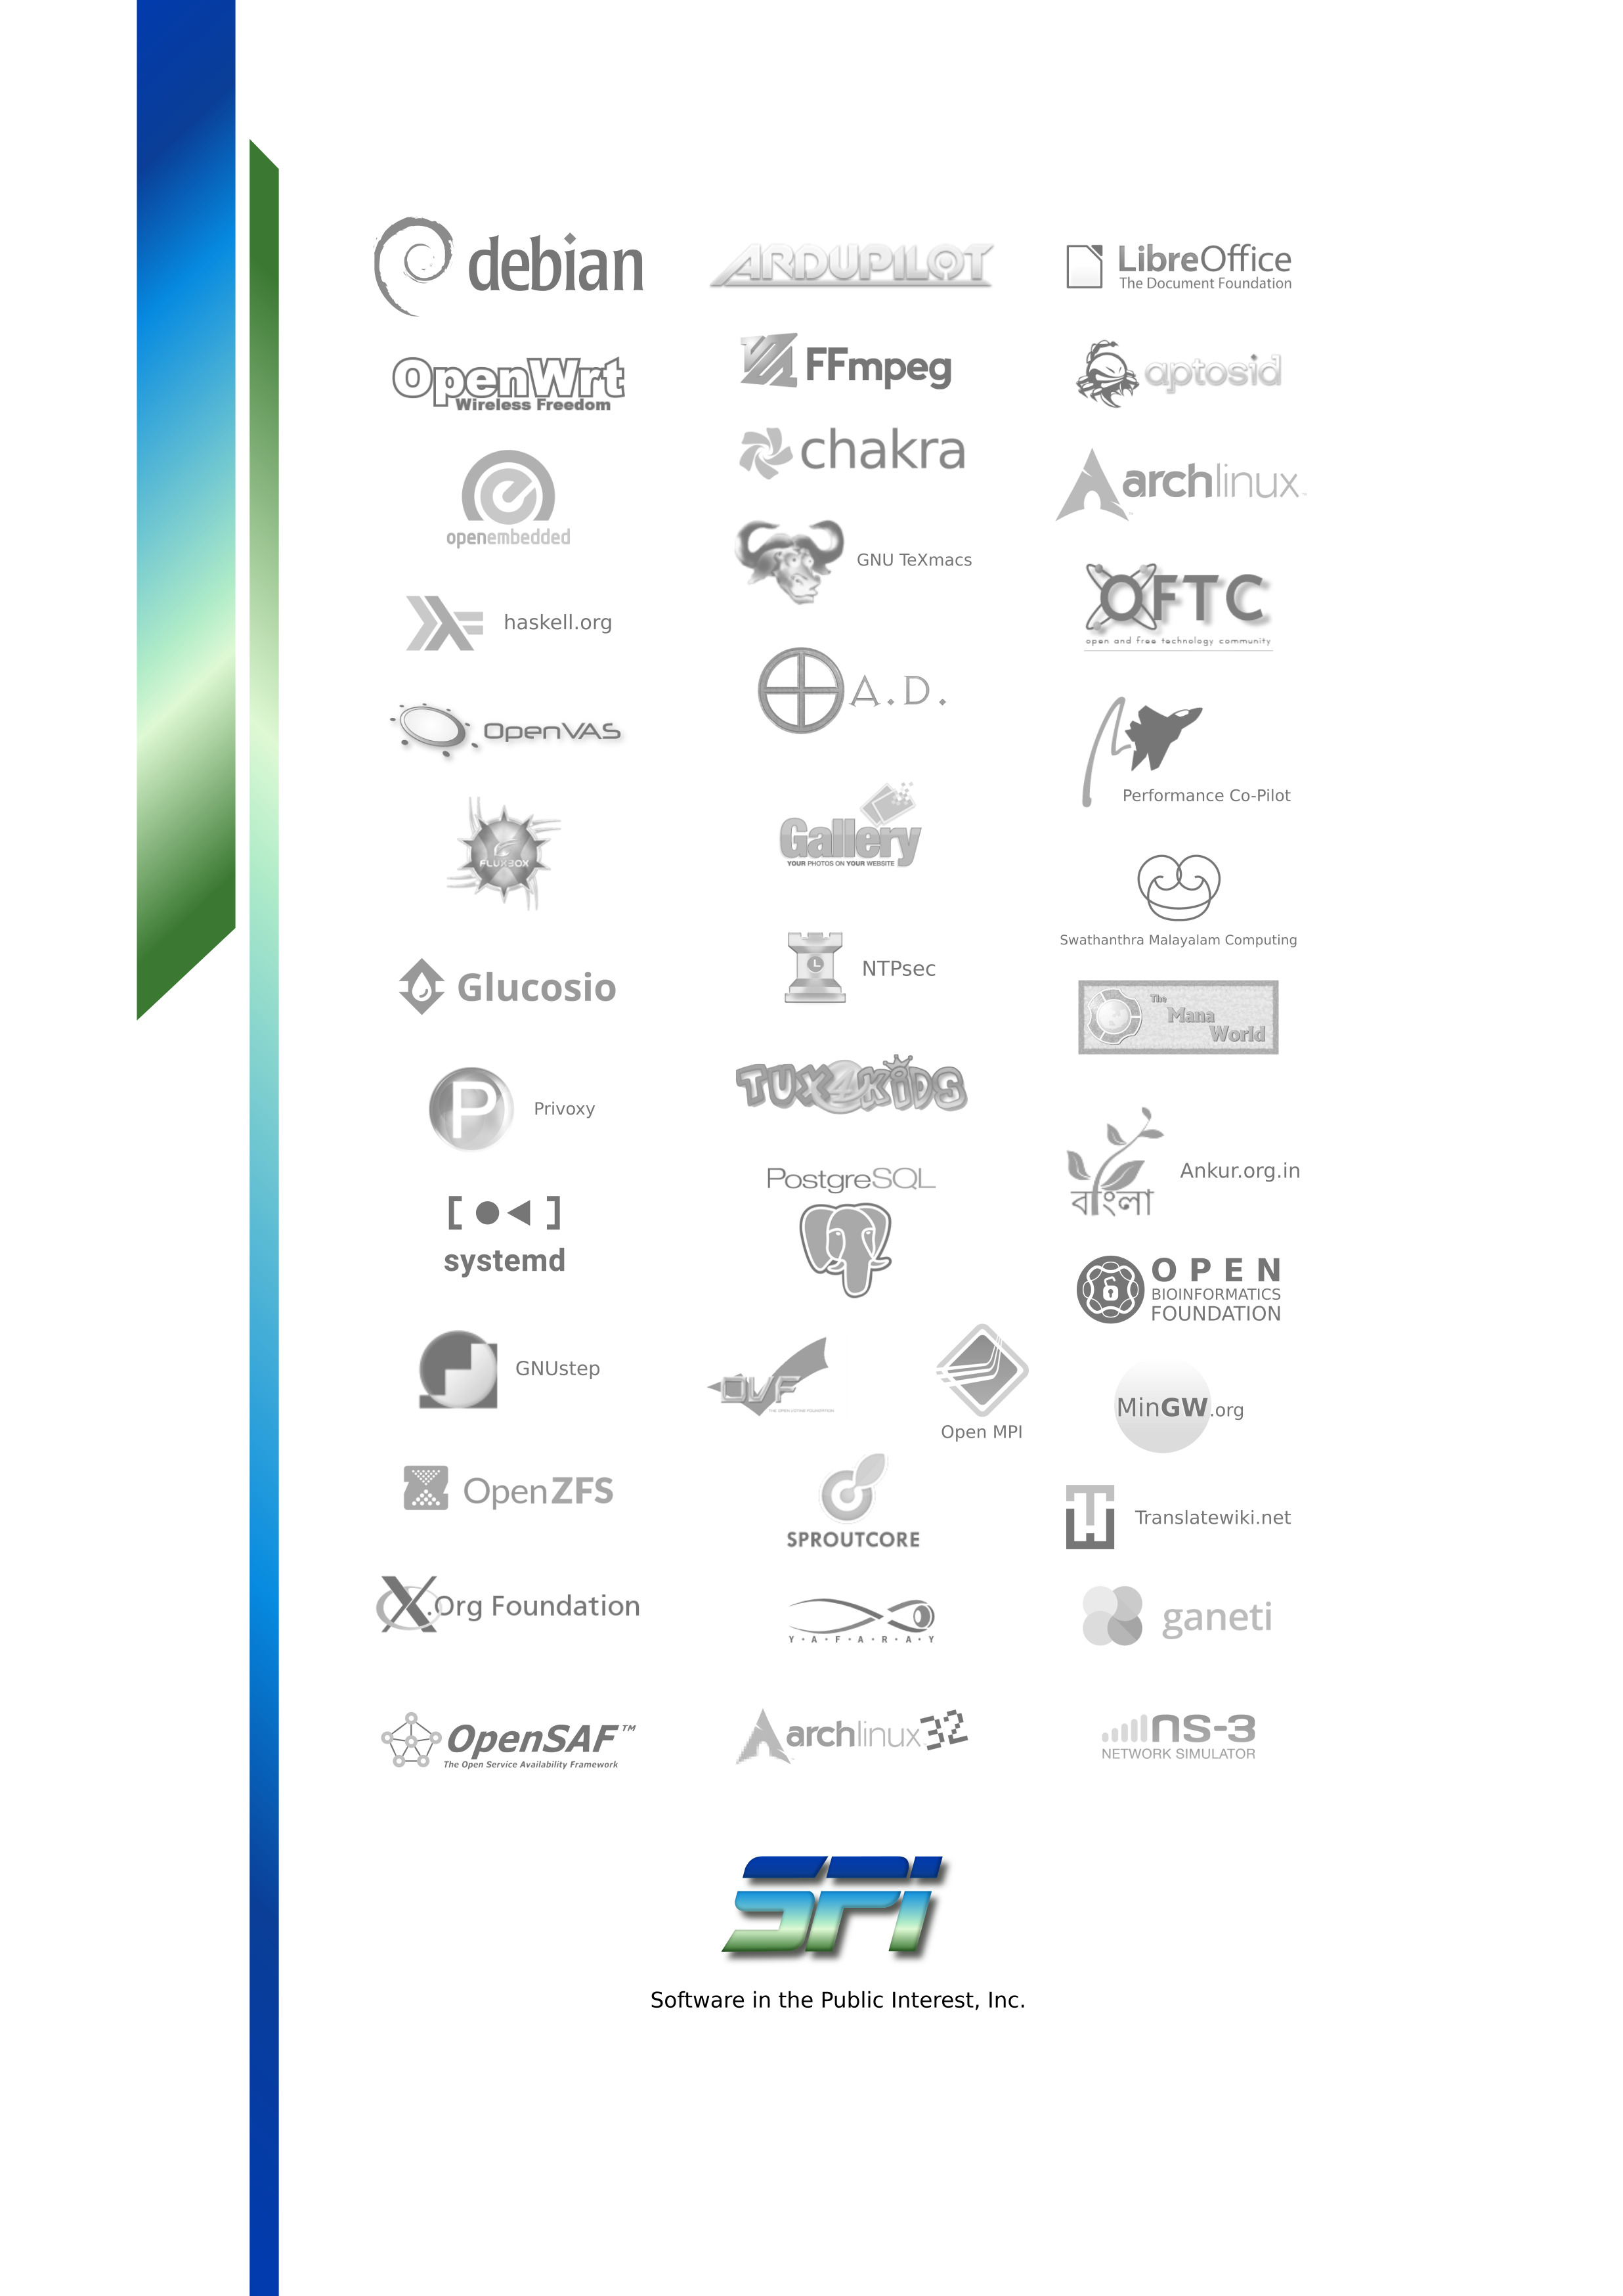
\includegraphics[width=\paperwidth,height=\paperheight]{images/spi-back-2020.jpg}}
}

\null

\end{document}
% Keep this at the bottom, thanks.
% Local Variables:
% TeX-master: "report"
% End:
